\chapter{Malayalam}
\section{Introduction}

Like many other Indic scripts, it is an abugida, or a writing system
that is partially “alphabetic” and partially syllable-based. The
modern Malayalam alphabet has 13 vowel letters, 36 consonant letters,
and a few other symbols. The Malayalam script is a Vattezhuttu script,
which had been extended with Grantha script symbols to represent
Indo-Aryan loanwords. The script is also used to write several
minority languages such as Paniya, Betta Kurumba, and Ravula. The
Malayalam language itself was historically written in several
different scripts.

As is the case for many other Brahmi-derived scripts in the Unicode
Standard, Malayalam uses a virama character to form consonant
conjuncts. The virama sign itself is known as candrakala({\meera ചന്ദ്രക്കല}) in
Malayalam.

When the candrakala sign is visibly shown in Malayalam, it usually
indicates the suppression of the inherent vowel, but it sometimes
indicates instead a reduced schwa sound, often called “half-u” or
samvruthokaram. In the latter case, there can also be a -u vowel sign,
and the base character can be a vowel letter. In all cases, the
candrakala sign is represented by the character U+0D4D Malayalam sign
virama, which follows any vowel sign that may be present and precedes
any anusvara that may be present.

FIXME samvruthokaram needs more explanation, refer
{\url{
http://thottingal.in/documents/Malayalam_Unicode_Report_of_Workshop_Kerala_Unive
rsity.pdf}}
and {\url{http://smc.org.in/doc/rachana-malayalam-collation.pdf}}

\section{Orthography variation}

Malayalam has two orthography variations, both actively
used. Generally they are known as Old orthography and Modern
orthography. Old orthography is also known as traditional
orthography. Modern orthography is also known as reformed orthography.

Old orthography is generally identified by large number of ligature
glyphs, often formed by more than one consonants or vowel
combination. For example, in old orthography, consonant {\meera ക} +
vowel { \meera ൂ} will form {\meera കൂ} as a single ligature. similarly a
conjunct {\meera ക + ് + ത} will form {\meera ക്ത} as a single
ligature. Font developers of traditional style fonts design and draw
this large set of glyphs. For a reference font Meera, the number of
glyphs is approximately over a thousand.

In the 1970's and 1980's, Malayalam underwent orthographic reform due to
printing difficulties. The treatment of the combining vowel signs u
and uu was simplified at this time. These vowel signs had previously
been represented using special cluster graphemes where the vowel signs
were fused beneath their consonants, but in the reformed orthography
they are represented by spacing characters following their consonants.


\begin{figure}[h]
   {\meera\large  മലയപ്പുലയനാ മാടത്തിന്‍മുറ്റത്തു\\
മഴ വന്ന നാളൊരു വാഴ നട്ടു.\\
മനതാരിലാശകൾപോലതിലോരോരോ \\
മരതകക്കൂമ്പു പൊടിച്ചുവന്നു.\\
അരുമക്കിടാങ്ങളിലൊന്നായതിനേയു -\\
മഴകിപ്പുലക്കള്ളിയോമനിച്ചു.}
   \caption{Text rendering using traditional orthography. Font used is Meera }
\end{figure}

\begin{figure}[h]
   {\lohitmalayalam\large  മലയപ്പുലയനാ മാടത്തിന്‍മുറ്റത്തു\\
മഴ വന്ന നാളൊരു വാഴ നട്ടു\\
മനതാരിലാശകൾപോലതിലോരോരോ \\
മരതകക്കൂമ്പു പൊടിച്ചുവന്നു\\
അരുമക്കിടാങ്ങളിലൊന്നായതിനേയു\\
മഴകിപ്പുലക്കള്ളിയോമനിച്ചു}
   \caption{Text rendering using modern orthography. Font used is Lohit
Malayalam}
\end{figure}

The above examples give high level difference in orthography.
Since both orthography is prominent in day to day usage of Malayalam, it will
be helpful to get more
understanding about the orthography variation. So let us go some more deep into
this differences.

For vowel signs, only u vowel({\meera ു}) and uu vowel({\meera ൂ})  make the
difference. {\meera ു}
\begin{figure}[h]
   Traditional: \\{\textexample{ \meera ക + ു = കു  \\
ക + ൂ = കൂ } }\\
 Modern:\\ \textexample{ \raghumalayalam ക + ു = കു \\
ക + ൂ = കൂ }\\
   \caption{Rendering difference of u and uu vowel signs}
\end{figure}

As you can see, in traditional orthography the vowel sign attach to the
consonant, while in modern script, the vowel sign is separate.

Reph sign varies in both orthographies. Reph sign is formed by VIRAMA+ RA i.e,
{\malayalam ് + ര}.
\begin{figure}[h]
Traditional:\\ {\meera\textexample  പ്ര }\\
Modern: \\ {\lohitmalayalam\textexample  പ്ര }
   \caption{Rendering difference of REPH sign}
\end{figure}

As you can see, in traditional orthography the reph sign attach to the
consonant, while in modern script,reph sign is separate and it get re-ordered
to the left of consonant.


\section{Reference fonts}

Since we need to illustrate both orthographies we will be using 2
fonts. For old orthography, we will use Meera font and for modern
orthography we will use Lohit Malayalam.

\subsection {Meera Font}
{\meera മീര മാതൃക }
// FIXME: Short introduction, designers, maintainers, usage info, popularity of
the font.

Meera font is maintained by Swathanthra Malayalam Computing initiative.

Homepage: {\url{https://savannah.nongnu.org/projects/smc}}

\subsection {Lohit Malayalam Font}
// FIXME: Short introduction, designers, maintainers, usage info, popularity of
the font.

\subsection {History}
In 2004, Red Hat released five Indian language fonts as open source licensed
under the GPL. In 2011, Red Hat re-licensed fonts under SIL OFL 1.1 license.
The fonts named Lohit which means Red in Sanskrit. Currently, the font family
supports 21 Indian languages: Assamese, Bengali, Devanagari (Hindi, Kashmiri,
Konkani, Maithili, Marathi, Nepali, Sindhi, Santali, Bodo, Dogri), Gujarati,
Kannada, Malayalam, Manipuri, Odiya, Punjabi, Tamil, and Telugu.

Now, Fedora Project and its contributors took the responsibility to consolidate
the further efforts and improvements of the Lohit fonts.

Homepage: {\url{https://fedorahosted.org/lohit/}}

\section{Technical details}
\subsection {Opentype Script Tags - mlym and mlm2}
\subsection {Reordering}
\subsection {Vowel signs and combining marks}

For every vowels except {\malayalam അ}, there are vowel signs in Malayalam

\begin{figure}[h]
  {\meera\textexample ‌ാ ി ീ ു ൂ ൃ ൄ െ േ ൈ ൊ ോ ൌ ൗ ം ഃ }\\
  \caption{Malayalam vowel signs.}
\end{figure}

The vowel signs cannot stand alone. It always applies to a consonant. To denote
that linguistic property, a dotted
rectangle appears if we try to render the vowel signs alone.

\begin{figure}[h]
  \centering
  {\meera\textexample ‌പ + ി =  പി }\\
  \caption{Malayalam vowel  {\malayalam ി} getting applied.}
\end{figure}

In the above shown vowel signs {\malayalam െ, േ, ൈ, ൊ, ോ, and ൌ } needs to be
reordered before rendering.
Rendering engines will reorder the glyphs before rendering and rendering engine
is aware of this property of the above vowels.
Inside the font, nothing special need to be done to get this reordering. Fonts
just need the glyph.

\begin{figure}[h]
  \centering
  {\meera\textexample ‌പ + െ =  പെ }\\
  \caption{Malayalam vowel  {\malayalam െ} getting applied after reordering.}
\end{figure}

vowel signs {\malayalam ൊ, ോ and ൌ} needs to be spit before rendering.
First part will be applied at the beginning of consonant cluster
and right part will be applied to end of consonant cluster. In rendering engine
terminology these vowel signs are known as "Split Matra".

\begin{figure}[h]
  {\meera\textexample ‌പ +  ൊ = പ + െ + ാ \\\\\
  = െ + പ + ാ \\\\
  = പൊ }
  \caption{Malayalam vowel  {\malayalam ൊ} getting spit and applied at left
and right of {\malayalam പ} .}
\end{figure}

In the above example, or in the rendering of split matra, the glyph mapped to
vowel signs {\malayalam ൊ, ോ and ൌ} has no role.
Whatever glyph present in the font for vowel signs {\malayalam ൊ, ോ and ൌ} will
not be used. Instead of that, glyphs mapped to the components after split will
be used. So what matters is what glyphs are mapped to vowel signs {\malayalam
‌ാ, െ, േ , ൗ  } matters.

Because of this, fonts will have glyphs to illustrate this process. For
example, Meera, Rachana fonts has the following drawing:

\begin{figure}[h]
  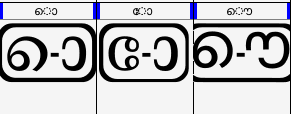
\includegraphics[width=0.8\textwidth]{images/malayalam-splitmatra-glyphs-meera.png}
  \caption{Split matra glyphs inside Meera font for  {\malayalam ൊ, ോ and ൌ}}
\end{figure}

We mentioned that dotted circles will appear left of the vowel sign if it is
not attached to consonant or consonant cluster.
But there are two known exceptions to this rule in Malayalam. One is
samvruthokaram.
In samvruthokaram - {\malayalam ു്} virama is applied to a vowel sign and this
can used to cause a rendering as shown in Figure \ref{WrongSamvruthokaram}.

\begin{figure}[h]
  \centering
  {\meera\textexample തു‌്}\\
  \caption{Wrong rendering of Samvruthokaram.}
  \label{WrongSamvruthokaram}
\end{figure}

This bug was fixed in 2008 and See section \ref{Samvruthokaram} on Samvruthokaram
for more details. It now renders properly as seen in Figure \ref{CorrectSamvruthokaram}.

\begin{figure}[h]
  \centering
  {\meera\textexample തു്}\\
  \caption{Correct rendering of Samvruthokaram.}
  \label{CorrectSamvruthokaram}
\end{figure}

Another exception is {\malayalam ാം}. This combination of a long vowel sign and
anusvara is used to denote "nth" like, {\malayalam 16ാം} or  {\malayalam 16-ാം}
meaning 16th. {\malayalam ാ} sign cannot appear in this example without a dotted
circle. To get the expected rendering, which is without dotted circle in this case,
Meera, Rachana and some other fonts has a trick. These fonts contains a special
glyph {\malayalam ാം}. This glyph is mapped to an akhand rule, see
Figure \ref{AkhandruleAAM}.

\begin{figure}[h]
  \centering
  {\meera\textexample  ാം = ◌ + ാ + ം}\\
  \caption{Akhand rule for {\malayalam ാം}. Dotted circle is included in the
rule.}
\label{AkhandruleAAM}
\end{figure}

\begin{figure}[h]
  \centering
  {\meera\textexample 16-ാം}\\
  \caption{16th with {\malayalam ാം} rendered correctly.}
  \label{CorrectAAMrendering}
\end{figure}

With this akhand rule, we will get expected rendering for "nth" patterns as
shown in Figure \ref{CorrectAAMrendering}.


You might have a question why dot is appearing for anusvara since that also
normally applied to a consonant cluster. But there are cases anusvara applied to
vowel signs as shown in figure \ref{Anusvararendering}.

\begin{figure}[h!]
  \centering
  {\meera\textexample നാലും, അടീം, ധൂം, ധിം, റാം, സ്റ്റെം, സ്റ്റോം}\\
  \caption{Anusvara {\malayalam ം} applied to a vowel sign.}
  \label{Anusvararendering}
\end{figure}

\subsubsection{Extra elongation for vowel signs}

Repeated vowel signs are used to denote elongation of a vowel pronunciation.
But rendering engines used to fail to render them properly because if vowel
signs are repeating, from second vowel sign onwards it is not attached to a
consonant cluster and it causes dotted circle. Now a days, Harfbuzz rendering
engine does not put dotted circle in between them. See Figures
\ref{elongatedvowel-dotted} and \ref{elongated-nodotted}.

\begin{figure}[h]
  \centering
  {\meera\textexample ടാാാാ}\\
  \caption{Repeated vowel signs.}
  \label{elongatedvowel-dotted}
\end{figure}

\begin{figure}[h]
  \centering
  {\meera\textexample ടാാാാാാാാ}\\
  \caption{Repeated vowel signs, dotted circle start appearing after 4th vowel sign.}
  \label{elongated-nodotted}
\end{figure}


\subsection {Samvruthokaram}
\label{Samvruthokaram}
Samvruthokaram is a mid vowel sound representation for vowel sign u. Now a
days, it is denoted just using virama like {\malayalam അത് ഉണ്ട് }, also known as
Pseudo Samvruthokaram
\footnote{Chandrakkala. Samvruthokaram. Chillaksharam.
From the perspective of Malayalam Collation
R. Chitrajakumar and N. Gangadharan
Rachana Akshara Vedi \url{http://www.unicode.org/L2/L2005/05210-malayalam.pdf}}
But using vowel sign of u and virama-{\malayalam ു്} to represent this is not
rare.

\begin{figure}[h!]
  \centering
  {\meera\textexample  അതു് ഉണ്ടു് }\\
  \caption{Rendering of Samvruthokaram with Meera font.}
  \label{SamvruthokaramTraditional}
\end{figure}

As you see, the vowel sign u attach to the consonant and virama appears on top.
With modern orthography the rendering is different, with different u and virama
signs explicitly shown as shown in Figure \ref{SamvruthokaramModern}.
Samvruthokaram rendering in traditional orthography is shown in Meera font in
Figure \ref{SamvruthokaramTraditional} for a comparison.

\begin{figure}[h!]
  \centering
  {\raghumalayalam\textexample  അതു് ഉണ്ടു് }\\
  \caption{Rendering of Samvruthokaram with Raghu Malayalam font.}
  \label{SamvruthokaramModern}
\end{figure}

It will look a bit odd to see these two signs in rendering in modern
orthography. In modern orthography samvruthokaram is very rare. Because of this
there was an attempt to add a glyph like virama to denote Samvruthokaram in
fonts like Raghu Malayalam and Lohit. But reverted recently(2013) since it
was quite an experiment. \footnote{Red Hat bugzilla:Samvruthokaram ligature is
wrong \url{https://bugzilla.redhat.com/show_bug.cgi?id=1013183}}

\subsubsection{History of Samvruthokaram rendering}

Samvruthokaram was one of the difficult rendering to get working in the initial
days of Malayalam computing. Rendering engines had the general concept that the
u vowel sign will not join with a virama. Of course Samvruthokaram was an
exception to that rule. Till 2009, this problem continued. Rendering engines
displayed samvruthokaram with dotted circled around Virama.
Volunteer developers from Swathanthra Malayalam Computing project worked
closely with Pango\footnote{\url{http://www.pango.org/}},
Qt\footnote{\url{http://qt-project.org}},
ICU\footnote{\url{http://userguide.icu-project.org/layoutengine}} rendering
engines to get the bug fixed.

Bug reports in respective bug tracking systems gives a detailed history of this
effort.

\begin{enumerate}
  \item Red Hat bug: \url{https://bugzilla.redhat.com/show_bug.cgi?id=242016}
  \item Pango Bug \url{https://bugzilla.gnome.org/show_bug.cgi?id=504810}
  \item ICU Bug \url{http://bugs.icu-project.org/trac/ticket/6108}
\end{enumerate}

\subsection {Conjunct Signs for യ, ര, ല}

Three consonants {\malayalam യ, ര, ല} has vowel like symbols in Malayalam.
These signs attach to the previous consonant cluster just like vowel signs.

\begin{figure}[h!]
  \centering
  {\meera\textexample ക് + യ = ക്യ \\ ക് + ര = ക്ര \\ ക് + ല = ക്ല }\\
  \caption{Rendering of consonant signs with Meera font.}
\end{figure}

\begin{figure}[h!]
  \centering
  {\raghumalayalam\textexample ക് + യ = ക്യ \\ ക് + ര = ക്ര \\ ക് + ല = ക്ല }\\
  \caption{Rendering of consonant signs with Raghu Malayalam font.}
\end{figure}

\subsection {Reph}
\subsection {Dot Reph}

Dot-Reph is used to represent Malayalam letter  {\meera ര} in its dead form
(or without vowel form), as a dot over the consonant following it.  It is
denoted by a dot on top of the letter. Dot reph is also known as Gopi Reph.
Usage of Dot Reph is not popular nowadays compared to the texts in past
decades.

\begin{figure}[h!]
  \centering
  {\meera\textexample ൎ }\\
  \caption{Dot Reph}
\end{figure}

The glyph can be circle shaped or in the form of a water drop upside down (also
known as a Gopi sign).

\begin{figure}[h!]
  \centering
  {\meera\textexample കര്‍ണ്ണന്‍  - കൎണ്ണന്‍ }\\
  \caption{Rendering of word കര്‍ണ്ണന്‍ without and with dotreph}
\end{figure}

In the above example, the word meaning remains same in both forms. The Dot Reph
was not encoded till Unicode version 5.1.

One of the reasons for not having an atomic code point in initial versions is that
it was considered as a typographer's choice to use it as a glyph variant for Chillu R.

In Unicode 5.1 this was encoded atomically with a code point 0D4E.
As per the proposal\footnote{ Dot Reph encoding proposal \url{http://std.dkuug.dk/jtc1/sc2/wg2/docs/n3676.pdf}},
the reason for encodings were given as

\begin{enumerate}
\item  {\malayalam ര + ് + ZWJ} is the natural choice for Dot Reph, but already used
for MALAYALAM CHILLU RR before Unicode 5.1. So if somebody want to use both
Chillu form and Dot Reph, it is impossible.
\item If {\malayalam ര + ് } is used for Dot Reph, it will conflict with the usual
usage of that sequence for words like {\malayalam ഭാര്യ, സൂര്യന്‍, കാര്യം } etc will break.
\item If {\malayalam റ + ് } is used for Dot Reph, In the words like
{\malayalam ഭാര്യ, സൂര്യന്‍, കാര്യം } etc, it is ര  that forms the conjuncts and not  {\malayalam റ}.
\end{enumerate}

Swathanthra Malayalam computing had opposed this proposal in the document they
submitted to Unicode \footnote{Atomic chillu's are Unacceptable L2/08-038 \url{http://wiki.smc.org.in/images/2/23/SMC_Unicode_5.1.pdf}}
with alternate way of representing Dot Reph without introducing a code point
difference to words with and without Dot Reph, as in the {\malayalam കര്‍ണ്ണന്‍}
example. Their proposal was to use Dot Reph if a font maps {\malayalam ര + ്  }
to a Dot Reph glyph or fallback to {\malayalam ര്‍} if the font does not have
the glyph. But this was not accepted and in Unicode 5.1, Dot Reph was encoded.

The Dot Reph appears as a dot above the subsequent Malayalam consonant or cluster.

\begin{figure}[h!]
  \centering
  {\meera\textexample ൎ + വ  = ൎവ }\\
  \caption{Rendering of {\malayalam ര്‍വ } using Dot Reph }
\end{figure}

More examples of words with Dot Reph is given below.

\begin{figure}[h!]
  \centering
  {\meera ഭാൎയ്യ സൂൎയ്യന്‍ കാൎയ്യം  കൎത്താവ്  ആൎക്ക്  വൎത്തുളം  സുഹാൎത്തോ}\\
  \caption{More Dot Reph examples}
\end{figure}

Rendering complexities of Dot Reph, with examples such as {\meera ആൎക്ക്  വൎത്തുളം  സുഹാൎത്തോ}.\\
Dot Reph is best implemented in font using Opentype Glyph Class 'Mark'. Base glyphs and conjuncts are not marked as 'Mark' class, but an Anchor point to those glyphs could be added indicating the position where Dot Reph would be placed.\\
Harfbuzz and Uniscribe reorders Dot Reph after the base glyph/conjunct. For instance \texttt{hb-shape} utility (from Harfbuzz source tree) shows the output of {\meera ൎത്തു} \texttt{<dotreph, th1, xx(virama), th1, u1(u-sign)>} as \\  \texttt{[th1th1u1=0+2461|dotreph=0\@-575,-5+0]}. Thus, it is only necessary to add an Anchor point to glyph \texttt{th1th1u1} at the desired coordinate to render dotreph.\\

An example of how to do this using Fontforge:
\begin{figure}[h!]
  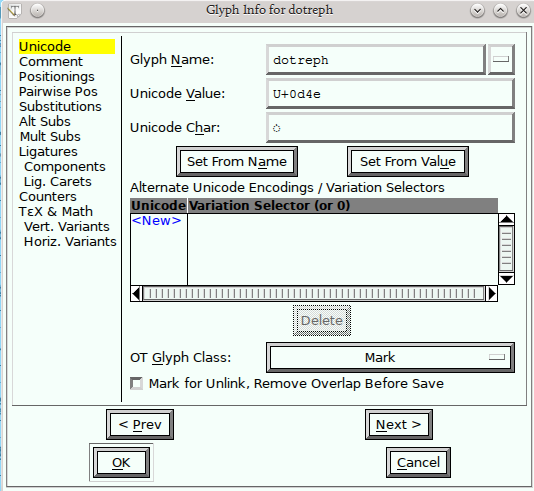
\includegraphics[width=0.5\textwidth]{images/malayalam-meera-dotreph-mark.png}
  \caption{Set OT Glyph Class of dotreph as 'Mark'}
\end{figure}
\begin{figure}[h!]
  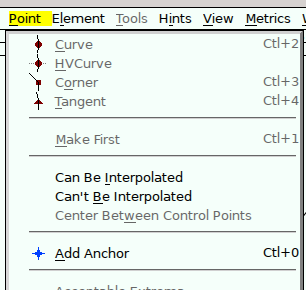
\includegraphics[width=0.3\textwidth]{images/malayalam-meera-conjunct-add-anchor.png}
  \caption{Add Anchor point menu}
\end{figure}
\begin{figure}[h!]
  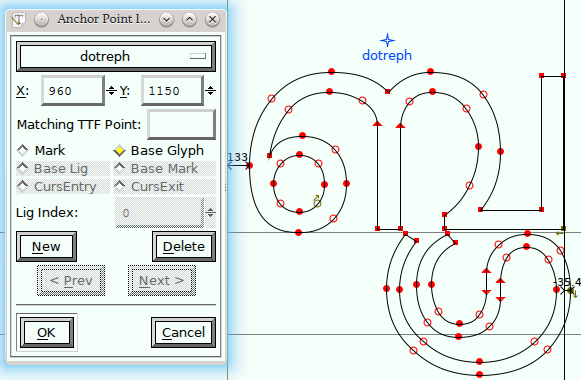
\includegraphics[width=0.65\textwidth]{images/malayalam-meera-conjunct-add-anchor-2.png}
  \caption{Position the dotreph Anchor point on the glyph}
\end{figure}


\subsection {Chillus}
\subsection {Stacking}
\subsection {Font metrics}
\subsection {Positioning rules}
\subsection {ZWNJ and ZWJ Signs}
\subsection {Prebase substitutions}
\subsection {Akhand forms}
\subsection {Below base forms}
\subsection {Below base substitutions}
\subsection {Half forms}
\subsection {Postbase forms}
\subsection {Latin glyphs and punctuations}
\subsection {Kerning}
\subsection {Shape references}
\subsection {Left and right bearings}
\subsection {Italic variant}
\subsection {Bold variant}

\section{Design}
\subsection{Number of glyphs}

The main difference between traditional and new orthography is the number of
glyphs to be designed and drawn for a font.
Traditional orthography fonts require more than 1000 glyphs while new orthograhy
fonts need less than 400 glyphs.

Meera font has around 1100 glyphs while Raghu Malayalam font has around 350
glyphs.

\subsection{Guidelines}

There is no rule about whether a particular glyph can be present only in
traditional font or new orthography font. It is up to the designer. But it is
possible to list certain guidelines about this.

\begin{enumerate}
\item Include basic punctuations. Punctuations can come inside Malayalam text.
To make the rendering consistent, punctuation marks that match the font style
should be present in the font.
\item Include Arabic numbers
\item All Malayalam characters encoded by the current Unicode version
\item Zero width joiner Zero width non-joiner place holder glyphs - TODO
explain in detail
\item A fall back glyph mapped to .notdef, usually a box
\item Dotted circle - To denote invalid combining marks, ie usually invalid
vowel signs at wrong positions, opentype specification
recommends to add a glyph of Unicode character U+25CC.
\footnote{Invalid combining marks.
\url{http://www.microsoft.com/typography/OpenTypeDev/malayalam/intro.htm}}
The glyph should be a
dotted circle. A few examples where they will be used is given below.
\begin{figure}[h]
  \centering
  {\meera\textexample ോ ു ി ുപ }\\
  \caption{Dotted circle example}
\end{figure}

Rendering engines can decide whether a vowel sign is at valid position or not
and implementation may vary.
One should not expect linguistic correctness on this. For example, a vowel sign
after a vowel is invalid for Malayalam, but following rendering does not show
dotted circle.

\begin{figure}[h]
  \centering
  {\meera\textexample ആാ ഊൂ }\\
  \caption{Rendering not showing dotted circle even though incorrect in
linguistic sense.}
\end{figure}

\item Malayalam glyphs with opentype feature tables
\item Rendering consistency - It will be easy to explain this with an example.
Consider the case of {\malayalam യ്ക}.The ka is stacked under ya. If a font has
this kind of stacking, the same font must have a number of additional glyphs to
make rendering consistent.
\begin{figure}[h!]
  \centering
  {\meera\textexample യ്ക യ്ക്ക യ്ക്കു യ്ക്കൂ }\\
  \caption{Consistent stacking of letters}
\end{figure}

If the designer miss to add {\meera യ്ക്ക യ്ക്കു യ്ക്കൂ }, the consistency will
be broken and it will render as follows:
\begin{figure}[h]
  \centering
  {\meera\textexample യ്ക യ്ക്‌ക യ്ക്‌കു യ്ക്‌കൂ }\\
  \caption{Inconsistent stacking of letters}
\end{figure}

It will also get broken if the font has  {\meera യ്ക്ക} but missed to add
glyphs for {\meera യ്ക്കു യ്ക്കൂ }.

\begin{figure}[h]
  \centering
  {\meera\textexample യ്ക യ്ക്ക യ്ക്ക‌ു യ്ക്ക‌ൂ }\\
  \caption{Inconsistent stacking of letters}
\end{figure}

If the font designer decides not to have glyph for {\meera യ്ക } at  all, none
of the above issues arise, but  {\meera യ്ക } is a common ligature in Malayalam.

In the last example, rendering is not broken if the font is a new orthography
font. But if it is a traditional orthography font, designer should make sure all
stacked glyphs are present in the font to provide consistent rendering. This is
one of the reason for lot of glyphs appearing in a traditional orthography font.

\begin{figure}[h]
  \centering
  {\meera\textexample സ്ക സ്കു സ്കൂ സ്കൃ \\ സ്ക്ര സ്ക്രു സ്ക്രൂ സ്ക്ക \\ സ്ക്കു സ്ക്കൂ സ്ക്കൃ }\\
  \caption{All glyph combinations of sa and ka stacked - from Meera font}
\end{figure}

\end{enumerate}
